\subsection{Validazione e collaudo}
Periodo: dal \textbf{2022-05-19} al \textbf{2022-06-07} \mbox{} \\ \mbox{} \\
La fase inizia appena conclusa la precedente e termina con la revisione \CA{} \\
Le precondizioni sono:
\begin{itemize}
 	\item aggiornamento e correzione dei documenti;
 	\item superamento del colloquio per la \PB{};
  	\item raggiungimento di un prodotto completo, funzionante e di qualità (secondo quanto stabilito nelle \NdP{} e nel \PdQ{} ) in ogni sua parte.
\end{itemize} \mbox{} \\
Le postcondizioni sono:
\begin{itemize}
	\item aggiornamento ed approvazione dei documenti prodotti precedentemente;
	\item esecuzione dei test di sistema e accettazione;
	\item completamento del prodotto software;
 	\item consegna della documentazione richiesta in entrata alla revisione \CA{}
	\item realizzazione della presentazione;
 	\item preparazione al collaudo.  
\end{itemize} \mbox{} \\
La fase è stata suddivisa in quattro incrementi di sviluppo.


\subsubsection{IX Incremento}
\subsubsubsection{Obiettivi}
Gli obiettivi che il gruppo si prepone per questo incremento sono:
\begin{itemize}
	\item completamento degli ultimi casi d'uso;
  	\item incremento della documentazione per verifica e miglioramento continuo.
\end{itemize}
\subsubsubsection{Periodo}
Il gruppo ritiene che il raggiungimento degli obbiettivi richiederà due settimane di lavoro, dal \textbf{2022-05-16} al \textbf{2022-05-29}.
\subsubsubsection{Ruoli attivi}
Per raggiungere gli obiettivi il gruppo ritiene che è necessario il lavoro delle seguenti figure:
\begin{itemize}
	\item \RE{};
 	\item \AM{};
   	\item \PT{};
    \item \PR{};
   	\item \VE{}.
\end{itemize}
\subsubsubsection{Attività}
Per raggiungere gli obiettivi preposti, il gruppo ritiene che dovranno essere svolte le seguenti attività:
\begin{itemize}
	\item \textbf{codifica:}
			\begin{itemize}
				\item implementazione UCW8 - Filtra classifica; requisiti:
					\begin{itemize}
						\item R1FW8;
						\item R1FW8.1;
						\item R2FW8.2;
						\item R2FW8.3;
						\item R2FW8.4;
      					\item R2FW8.5
					\end{itemize}
				\item implementazione UCW9 - Modifica parametri di ordinamento classifica; requisiti:
					\begin{itemize}
						\item R3FW9;
						\item R3FW9.1;
						\item R3FW9.2;
					\end{itemize}
			\end{itemize}
 	\item \textbf{verifica:} rilevazione metriche di qualità di prodotto e di processo;
	\item \textbf{documentazione:} 
	 \begin{itemize}
		\item integrazione del \MU{} in base alle nuove funzionalità implementate;
  		\item integrazione del \MA{} in base alle nuove funzionalità implementate;
		\item compilazione del \G{};
  		\item registrazione dei test di validazione;
    	\item registrazione degli esiti della verifica;
     	\item registrazione dell’andamento degli obiettivi di qualità;
      	\item aggiornamento della classificazione e rilevazione dei rischi;
		\item aggiornamento delle valutazioni per il miglioramento; 
		\item calcolo del preventivo a finire rispetto alla fase;
  		\item calcolo del consuntivo di periodo;
		\item calcolo del preventivo a finire rispetto al completamento del progetto.
	 \end{itemize}
\end{itemize}
\subsubsubsection{Diagramma di Gantt}

% \begin{figure}[H]
% 	\centering
% 	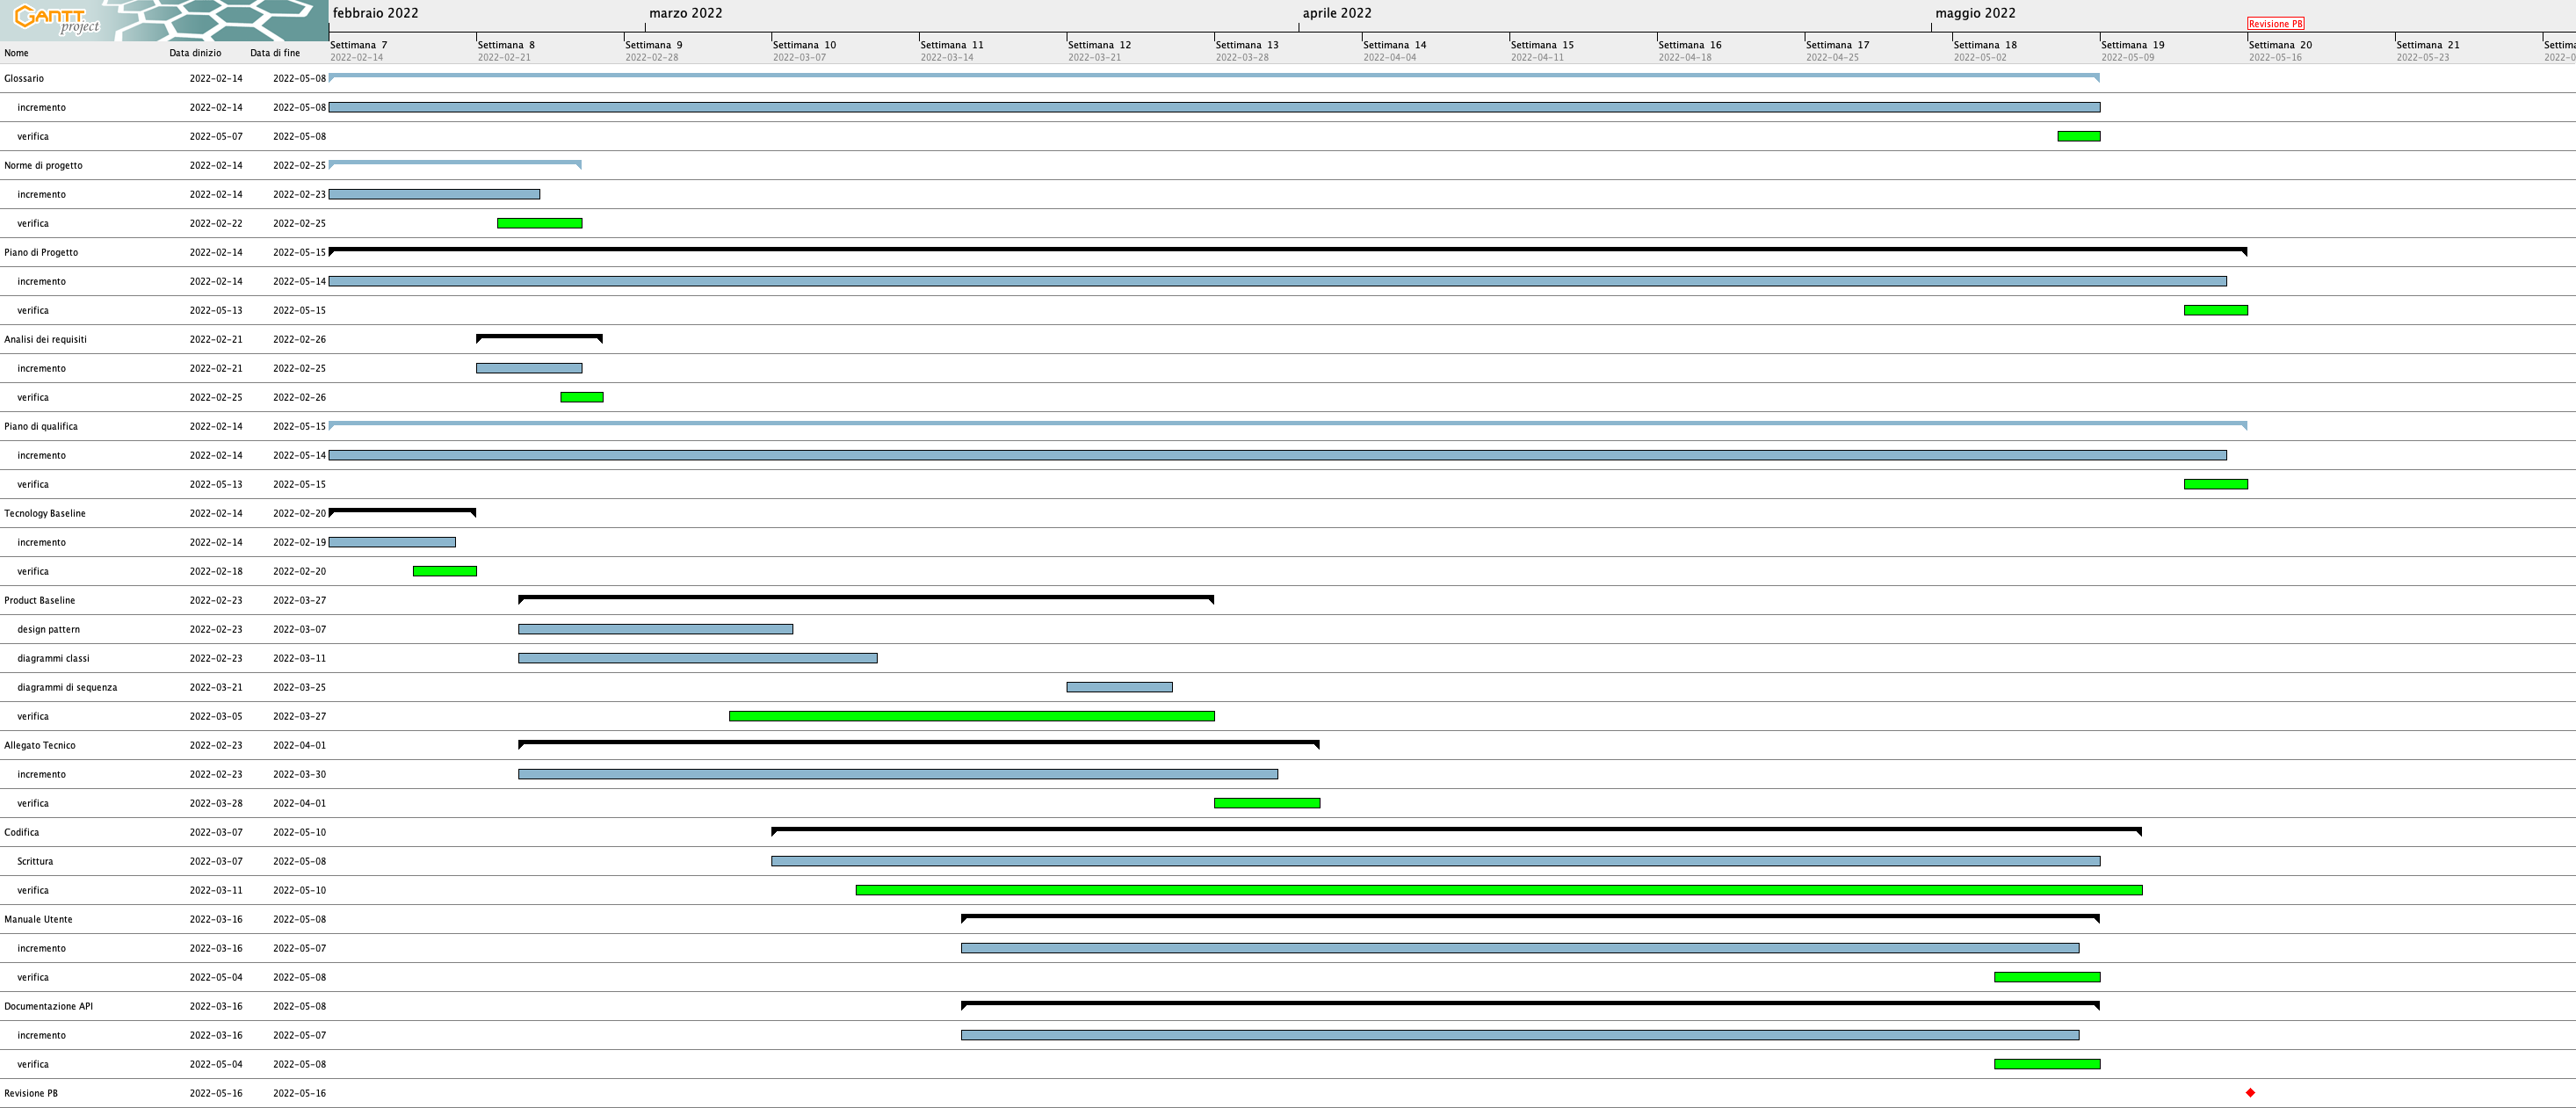
\includegraphics[scale=0.35]{Sezioni/gantt/progettazione_codifica.png}
% 	\caption{Diagramma di Gantt - Progettazione e codifica}
% \end{figure}

\subsubsection{X Incremento}
\subsubsubsection{Obiettivi}
Gli obiettivi che il gruppo si prepone per questo incremento sono:
\begin{itemize}
	\item miglioramento del sistema di assegnazione dei punteggi nella classifica;
  	\item incremento della documentazione per verifica e miglioramento continuo;
	  \item preparazione all’esposizione della revisione \CA{};
  	\item preparazione della lettera di presentazione.
\end{itemize}
\subsubsubsection{Periodo}
Il gruppo ritiene che il raggiungimento degli obbiettivi richiederà circa due settimane di lavoro, dal \textbf{2022-05-30} al \textbf{2022-06-15}.
\subsubsubsection{Ruoli attivi}
Per raggiungere gli obiettivi il gruppo ritiene che è necessario il lavoro delle seguenti figure:
\begin{itemize}
	\item \RE{};
 	\item \AM{};
   	\item \PT{};
    \item \PR{};
   	\item \VE{}.
\end{itemize}
\subsubsubsection{Attività}
Per raggiungere gli obiettivi preposti, il gruppo ritiene che dovranno essere svolte le seguenti attività:
\begin{itemize}
	\item \textbf{codifica:}
			\begin{itemize}
				\item implementazione UCW8 - Filtra classifica; requisiti:
					\begin{itemize}
						\item R1FW8;
						\item R1FW8.1;
						\item R2FW8.2;
						\item R2FW8.3;
						\item R2FW8.4;
      					\item R2FW8.5
					\end{itemize}
				\item implementazione UCW9 - Modifica parametri di ordinamento classifica; requisiti:
					\begin{itemize}
						\item R3FW9;
						\item R3FW9.1;
						\item R3FW9.2;
					\end{itemize}
			\end{itemize}
 	\item \textbf{verifica:} rilevazione metriche di qualità di prodotto e di processo;
	\item \textbf{documentazione:} 
	 \begin{itemize}
		\item integrazione del \MU{} in base alle nuove funzionalità implementate;
  		\item integrazione del \MA{} in base alle nuove funzionalità implementate;
		\item compilazione del \G{};
  		\item registrazione dei test di validazione;
    	\item registrazione degli esiti della verifica;
     	\item registrazione dell’andamento degli obiettivi di qualità;
      	\item aggiornamento della classificazione e rilevazione dei rischi;
		\item aggiornamento delle valutazioni per il miglioramento; 
		\item calcolo del preventivo a finire rispetto alla fase;
  		\item calcolo del consuntivo di periodo;
		\item calcolo del preventivo a finire rispetto al completamento del progetto.
	 \end{itemize}
\end{itemize}
\subsubsubsection{Diagramma di Gantt}

% \begin{figure}[H]
% 	\centering
% 	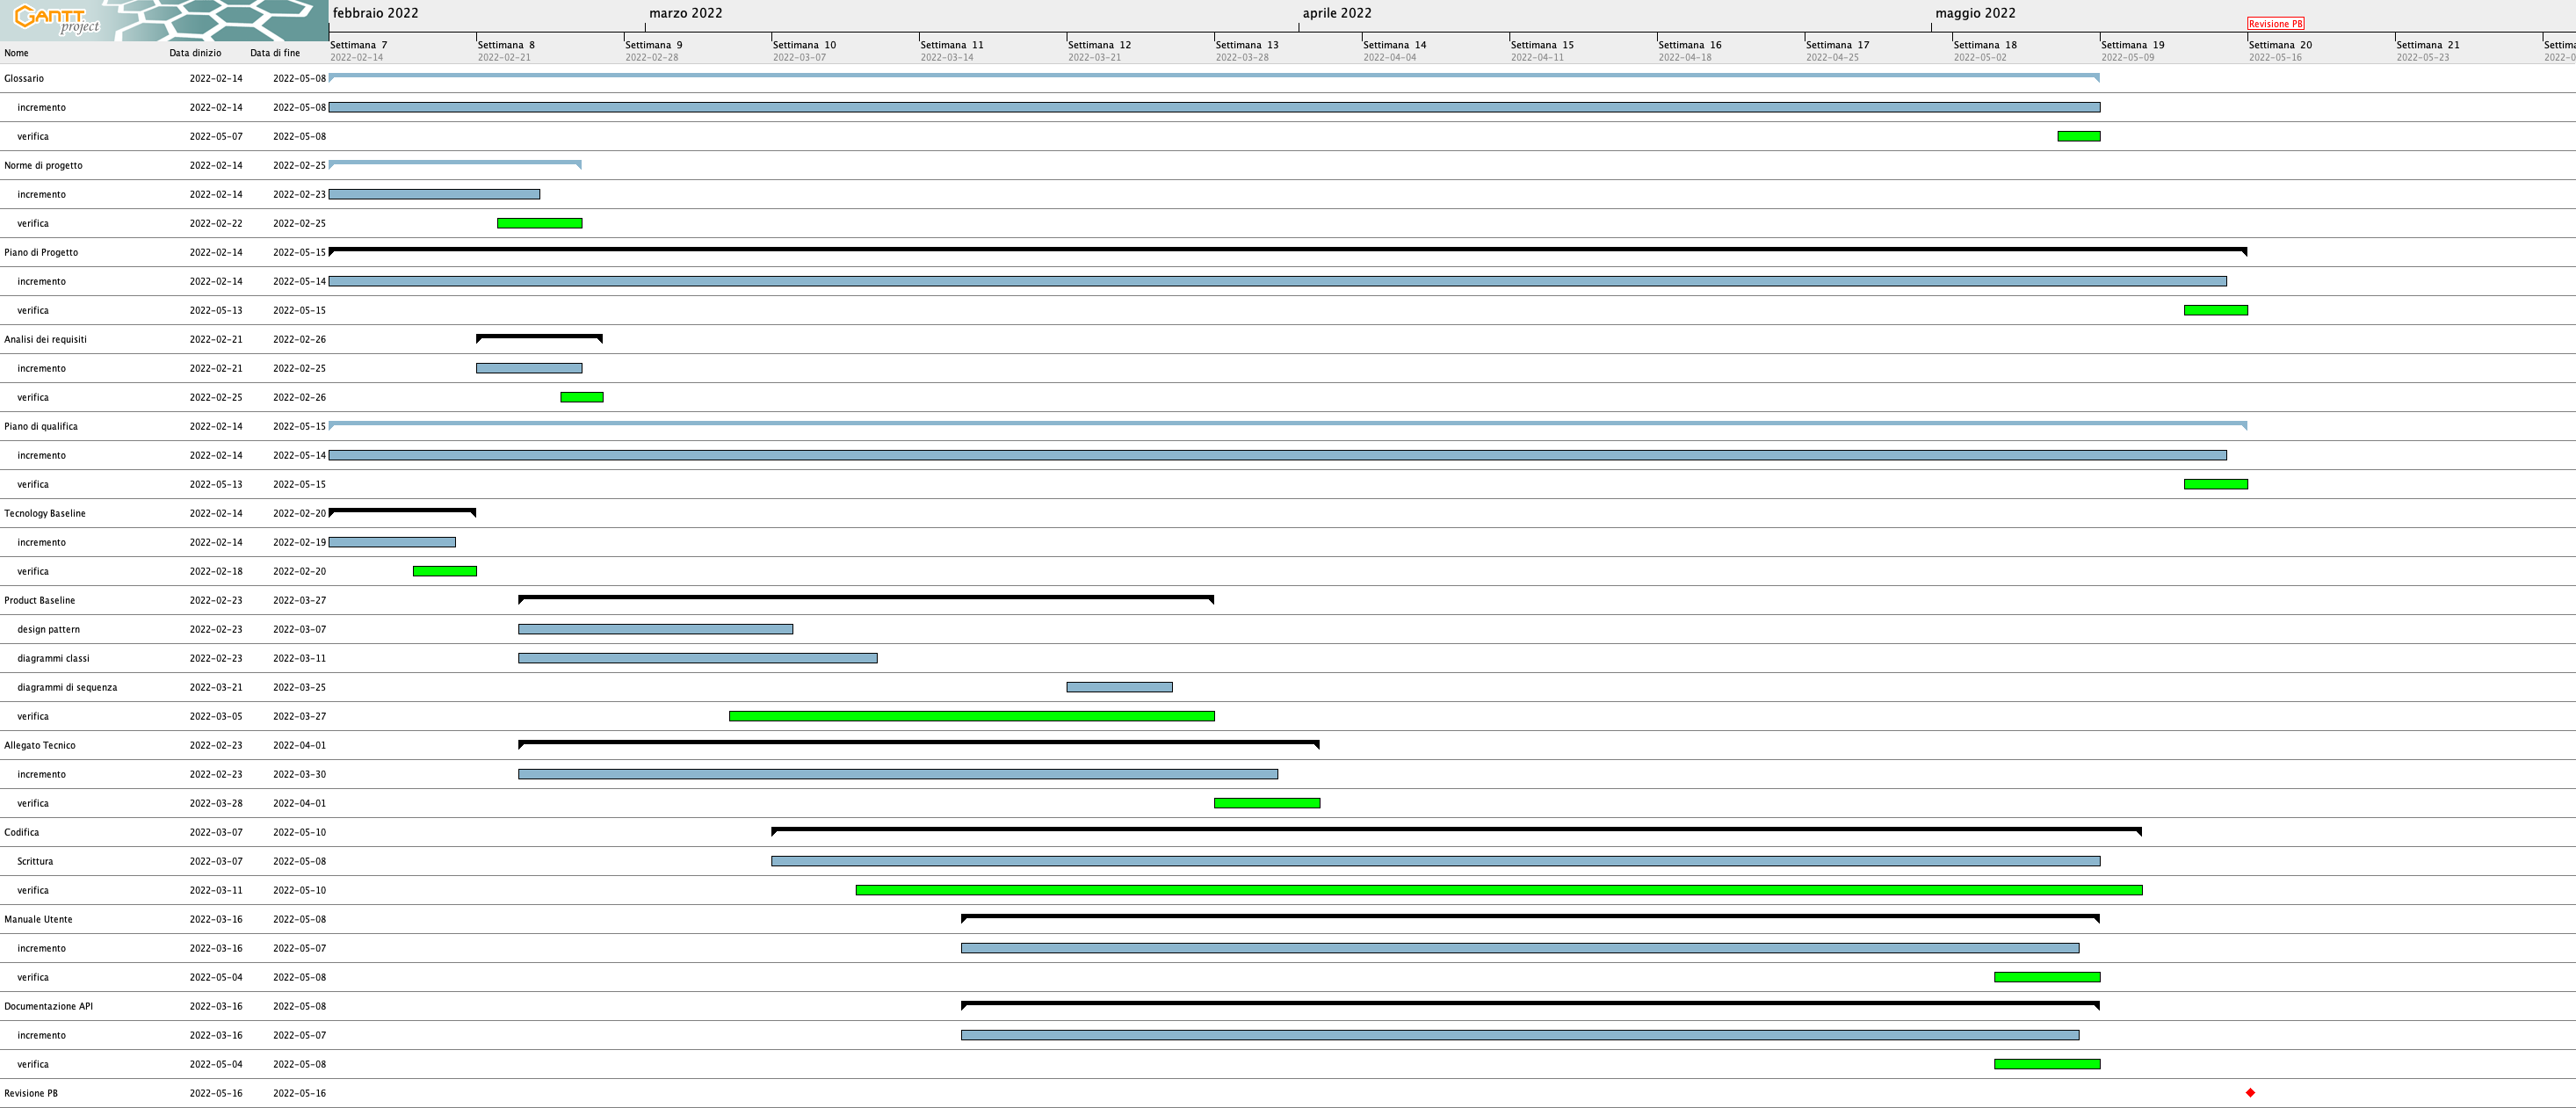
\includegraphics[scale=0.35]{Sezioni/gantt/progettazione_codifica.png}
% 	\caption{Diagramma di Gantt - Progettazione e codifica}
% \end{figure}







